% Chapter 2

\chapter{Abstraktes Beispiel} % Main chapter title

\label{Chapter2} % For referencing the chapter elsewhere, use \ref{Chapter2} 

Objektorientierte Programmiersprachen speichern Attribute und Methoden in Objekten, wehrend relationale Datenbanken ihre Daten in flachen Tabellen speichert. Aufgrund dieser beiden unterschiedlichen Konzepte entsteht ein Konzeptioneller Wiederspruch auch als object-relational impedance missmatch bekannt.

\begin{figure}[h]
\begin{center}
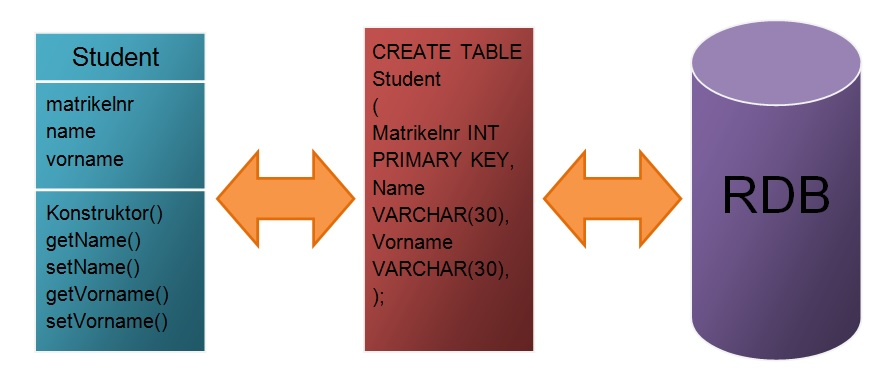
\includegraphics[width=1.0\textwidth]{ORM_Bild1.jpg}
\end{center}
\end{figure}

\newpage
Um diesen Widerspruch weit möglichst aufzulösen haben sich ORMs etabliert diese bieten den Vorteil das keine SQL Statements mehr im Programmcode notwendig sind, da diese vom ORM Framework automatisch generiert werden. Ein weiterer Vorteil ist das die Programmiersprache selbst nicht erweitert werden muss, da die Implementierung normalerweise über Klassenbibliotheken abgewickelt wird.

\begin{figure}[h]
\begin{center}
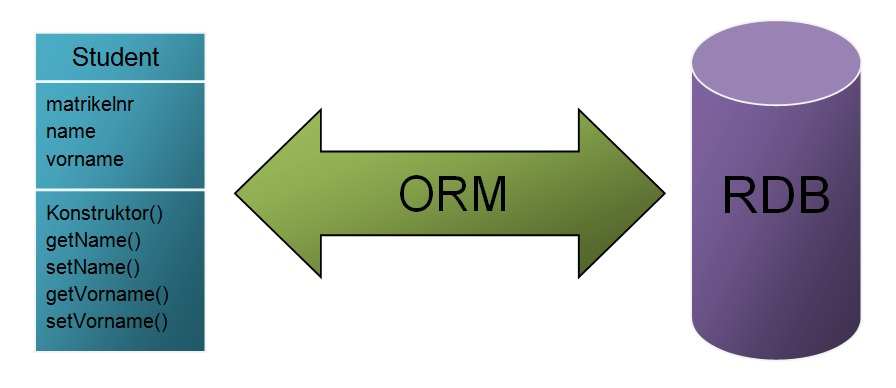
\includegraphics[width=1.0\textwidth]{ORM_Bild2.jpg}
\end{center}
\end{figure}
